\documentclass[10pt]{article}
\usepackage{graphicx}
\usepackage{algorithm}
\usepackage{algpseudocode}
\usepackage{siunitx}

\begin{document}
\title{CSE616 Neural Networks and Their Applications\\
Assignment 1 Submission}
\author{Ayman Wagih Mohsen (2000728)}
\maketitle

\section{Question 1}
An image of shape [3, 500, 500] is flattened to a vector of shape [750000, 1]. A fully connected layer to 100 units has weights of shape [100, 750000], with bias of shape [100, 1]. There are (750000+1)*100 = 75000100 learned parameters.
\section{Question 2}
An image of shape [3, 500, 500] is sent to 10 filters of 5x5. The filters have weights of shape [10, 3, 5, 5] with bias of shape [10, 1, 1, 1]. There are (3*5*5+1)*10 = 760 learned parameters.
\section{Question 3}
The bottom left image shown below was run through a vertical edge detection filter, which has a high pass filter effect in horizontal direction, and low pass filter in the vertical direction.\\

So it has the weights similar to:
\[
	\left[
	{
		\begin{array}{ccc}
		-1&0&1\\
		-1&0&1\\
		-1&0&1\\
		\end{array}
	}
	\right]
\]
The bottom right image was run through a horizontal edge detection filter, which is the previous filter taken sideways:
\[
	\left[
	{
		\begin{array}{ccc}
		-1&-1&-1\\
		0&0&0\\
		1&1&1\\
		\end{array}
	}
	\right]
\]
\begin{center}
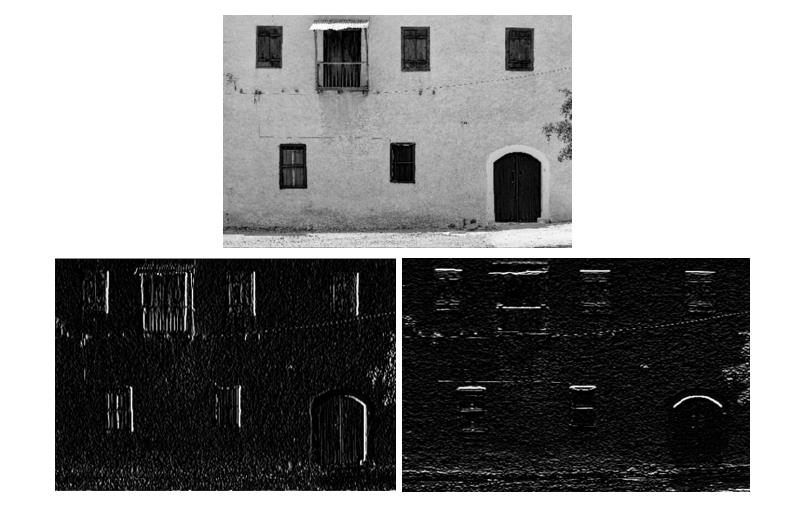
\includegraphics[width=0.9\textwidth]{20220502 Q3.PNG}
\DeclareGraphicsExtensions{.png}
\end{center}

\section{Question 4}
The Adam optimizer uses an exponential moving aveage filter to have a low pass filter effect on the mean and variance of the gradient.
\[
	variable:=variable*\alpha+update*(1-\alpha)
\]
Where $0<\alpha<1$ is close to 1.
To make the exponential moving average larger, set $\alpha$ closer to one.
The closer the alpha to unity, the stronger is the low pass filter effect.
When $\alpha$ is exactly one, variable will remain constant.

\begin{algorithm}
\caption{Adam optimizer initialization}\label{euclid}
\begin{algorithmic}[1]
\Procedure{Adam\_initialization}{}
\State $m=0$
\State $v=0$
\State $\alpha=0.001$
\State $\beta_1=0.9$
\State $\beta_2=0.999$
\EndProcedure
\end{algorithmic}
\end{algorithm}

\begin{algorithm}
\caption{Adam optimizer iteration}\label{euclid}
\begin{algorithmic}[2]
\Procedure{Adam\_iteration}{}
\State $grad:=compute\_gradient()$
\State $m:=\beta_1 m+(1-\beta_1)grad$
\State $v:=\beta_2 v+(1-\beta_2)grad^2$
\State $\hat{m}:=\frac{m}{1-\beta_1^t}$
\State $\hat{v}:=\frac{v}{1-\beta_2^t}$
\State $w:=w-\alpha\frac{\hat{m}}{\sqrt{\hat{v}}+\num{1e-8}}$
\EndProcedure
\end{algorithmic}
\end{algorithm}

\section{Question 5}
With m features $(z^{(1)}, ..., z^{(m)})$ and a size n batch of training data, we calculate the mean and variance of each feature over the batch:
\[	\mu=\frac{1}{m}\sum_{i=1}^{m}x_i\]
\[	\sigma^2=\frac{1}{m}\sum_{i=1}^{m}(x_i-\mu)\]
Then each component $k^{th}$ in the input is normalized with its mean and variance:
\[	\hat{z}_i^{(k)}=\frac{x_i^{(k)}-\mu^{(k)}}{\sqrt{{\sigma^{(k)}}^2+\epsilon}}\]
Then each $k^{th}$ component is scaled and shifted by $k^{th}$ learned parameters $\gamma$ and $\beta$:
\[	y_i^{(k)}=\gamma^{(k)}\hat{x}_i^{(k)}\beta^{(k)}\]
Batch normalization is needed when the features $z^{(k)}$ have wildly different ranges resulting in the dimensions of the scalar field being stretched differently, causing the optimizer to go in a zigzag pattern. Also, by using batch normalization, a higher learning rate can be used.

\section{Question 6}
\begin{tabular}{|l|c|c|c|c|c|c|}
	Layer & Input & Filter & Padding & Stride & Output & Field\\
	conv1 & 3*256*256 & (3*3*3+1)*32 & 1 & 1 & 32*256*256 & 3*3\\
	pool & 32*256*256 & - & 0 & 2 & 32*128*128&2*2\\
\end{tabular}
\\
\\The combined receptive field is 4*4.

\section{Question 7}
The output has the number of channels equal to the number of filters, and the dimensions are given by:
\[
	D_{out}=\frac{D_{in}+2P-F}{S}+1
\]
Therefore the output shape is 128 channels of 64*64.

\section{Question 8}
Inverted dropout is a compensation for the summation of nodes by the ratio of nodes that were kept to the total number of nodes. For example if there are 10 nodes in layer 1, and 5 nodes were dropped. Then the input to layer 2 should be multiplied by 1/2 at test time, where all nodes are used. To avoid this, inverted dropout is used: we divide the nodes by the dropout probability at train time instead. So that we don't have do do anything at test time.

\section{Question 9}
Fully connected (FC) layers don't work well for image classification because they have an impractically large number of learned parameters per layer, which is approximately the product of all input and output dimensions. FC layers also don't consider the spatial correlation found in images and treat each pixel as an independent input.

\section{Question 10}
The steps of the convolution are shown below. Note: the small input array was flipped. The result array is (-8, 2, 3, -7, 3).
\begin{center}
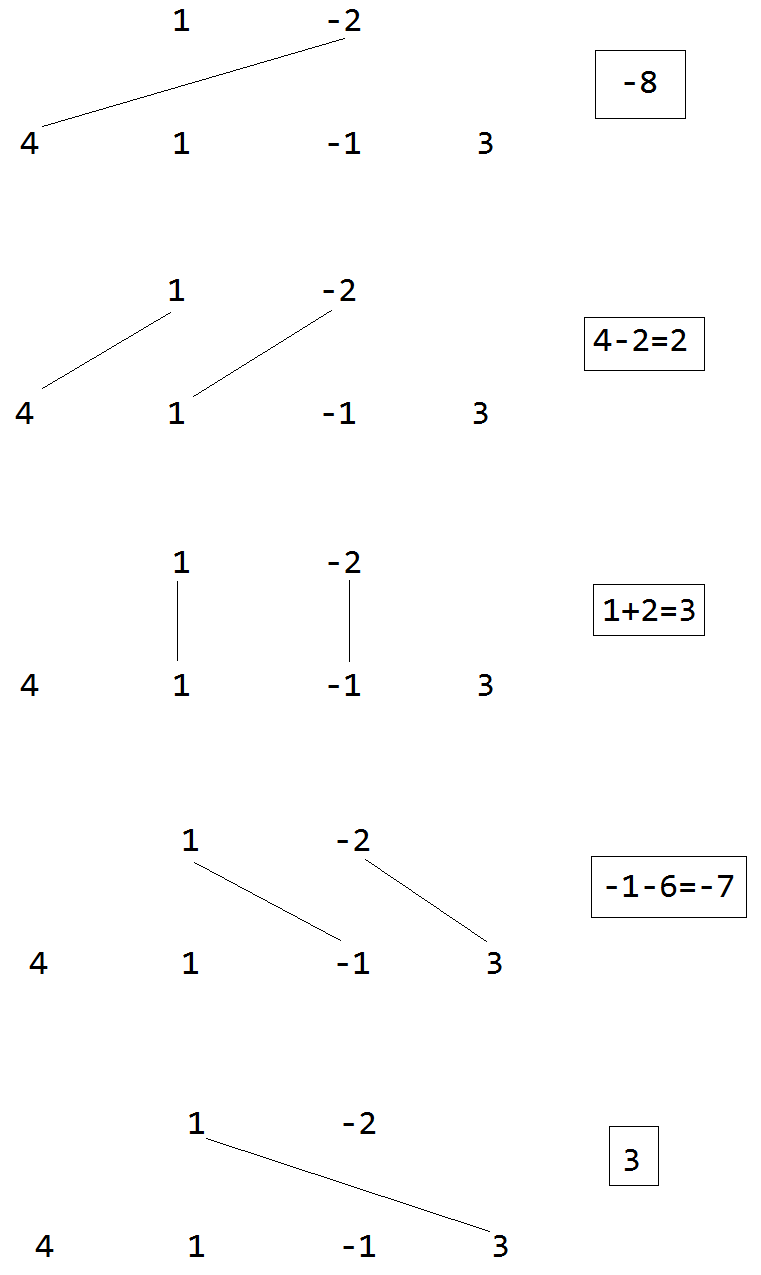
\includegraphics[width=0.9\textwidth]{20220503 Q10.PNG}
\DeclareGraphicsExtensions{.png}
\end{center}

\section{Question 11}
The optimizer passed through saddle point. At first, it converges down slowly to the saddle point, but then the gradient changes direction and it goes down fast in another direction.

\section{Question 12}
Convolutional layers can extract features regardless of their position in the image, and they usually have less learned parameters than comparable fully connected layers.

\section{Question 13}
There are two alternatives: The first is to multiply all hidden nodes that were subject to dropout by p at test time only. The second, better alternative is to divide retained hidden nodes by p at train time. This is to compensate the lesser sum at train time than at test time due to dropout. 

\section{Question 14}
The difference between standard momentum optimizer and Nesterov optimizer is that in standard momentum the gradient is calculated at current position, then we update the velocity, then we jump to a new position according to new velocity. While in Nesterov optimizer, we first predict where we will be accodding to previous velocity and calculate the gradient at the predicted location. Then we update the velocity. Then we jump from the position at start of iteration according to the new velocity. Because the gradient is calculated at the destination of the jump rather than at the source, this usually decreases the overshoots, and hence the optimizer converges faster.

\begin{center}
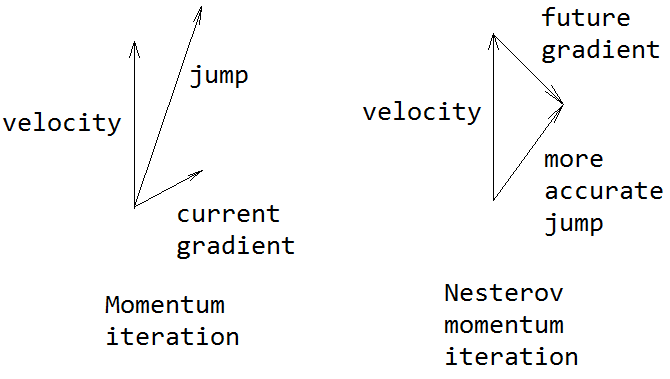
\includegraphics[width=0.9\textwidth]{20220504 Q14 Nesterov.PNG}
\DeclareGraphicsExtensions{.png}
\end{center}

\begin{algorithm}
\caption{Momentum optimizer}\label{euclid}
\begin{algorithmic}[2]
\Procedure{Momentum\_iteration}{}
\State $grad:=compute\_gradient()$
\State $v:=\alpha\times v+grad$
\State $w:=w-rate\times v$
\EndProcedure
\end{algorithmic}
\end{algorithm}

\begin{algorithm}
\caption{Nesterov optimizer}\label{euclid}
\begin{algorithmic}[2]
\Procedure{Nesterov\_iteration}{}
\State $grad:=compute\_gradient()$
\State $v2:=v$
\State $v:=\alpha\times v-rate\times grad$
\State $w:=w-\alpha\times v2+(1+\alpha)\times v$
\EndProcedure
\end{algorithmic}
\end{algorithm}

\section{Question 15}
In Adagrad optimizer, the gradient is element-wise multiplied by a variable factor. This factor is the learning rate divided by the square root of the gradient square plus a small epsilon (All operations here are element-wise).
\[	s_{i}:=s_{i}+grad_{i}^2\]
\[	factor_i:=\frac{rate}{\sqrt{s_{i}+\epsilon}}\]
\[	x_{i}:=x_{i}+factor_i\times grad_{i}\]
This has the effect as if the learning rate is normalizing the gradient components, and decreases with time. Because $s_i$ is accumulating the square of the gradient, which is always nonnegative. Dividing the original learning rate by $\sqrt{s_i+\epsilon}$ greatly decreases the learning rate for a component i whose partial derivative squared sum is big (progress slow in steep directions), and increases the learning rate is the gradient magnitude was consistently small (progress faster in shallow directions). And because the sum s can only increase, the learning rate decreases with iteration steps.

\end{document}
